% -*-mode: Latex-*-
% !TEX root = gen_tikz.tex
% authors: simon
%
% file: gen_tikz.tex
% contents: helper file to generate pdf files out of tikz pictures
% Sccs-Id: %W% %G%

\documentclass{article}
\usepackage{tikz}
\usetikzlibrary{automata,positioning,shapes,arrows,fit,external,calc}
\usetikzlibrary{decorations.pathmorphing}
\tikzexternalize % activate!
% \tikzset{external/force remake}
\begin{document}
\tikzstyle{box}=[rectangle, inner sep=5mm, draw=black!100]
\tikzstyle{boxr}=[rectangle, inner sep=3mm, draw=black!100, rounded corners]
\tikzstyle{boxbg}=[fill=black!10, rounded corners]
\tikzstyle{tf}=[double,decorate,decoration={snake,amplitude=.4mm,segment length=2mm,pre length=2mm,post length=2mm}]
\tikzstyle{tb}=[dashed]
\tikzstyle{fifo}=[double]
\tikzstyle{2up}=[yshift=2mm]
\tikzstyle{2down}=[yshift=-2mm]
\tikzstyle{2left}=[xshift=-2mm]
\tikzstyle{2right}=[xshift=2mm]

% ============================= ecm.tex =======================================
% Process network modelling a crossroad
\tikzsetnextfilename{cross_proc_dl}
\begin{tikzpicture}[shorten >=1pt,node distance=2cm,on grid,auto]
    \node[box] (NW) {$P_{\mathit{NW}}$};
    \node[box] (NE) [right of=NW, xshift=1cm] {$P_{\mathit{NE}}$};
    \node[box] (SW) [below of=NW, yshift=-0.5cm] {$P_{\mathit{SW}}$};
    \node[box] (SE) [right of=SW, xshift=1cm] {$P_{\mathit{SE}}$};
    \coordinate[right of=NE] (WO);
    \coordinate[left of=NW] (WI);
    \coordinate[left of=SW] (EO);
    \coordinate[right of=SE] (EI);
    \coordinate[above of=NW] (SO);
    \coordinate[below of=SW] (SI);
    \coordinate[below of=SE] (NO);
    \coordinate[above of=NE] (NI);
    \path[->] (WI) edge node {$m_{wi}$} (NW.west) (NW.east) edge node {$m_{w}$} (NE.west) (NE.east) edge node {$m_{wo}$} (WO);
    \path[->] (EI) edge node[swap] {$m_{ei}$} (SE.east) (SE.west) edge node[swap] {$m_{e}$} (SW.east) (SW.west) edge node[swap] {$m_{eo}$} (EO);
    \path[->] (NI) edge node {$m_{ni}$} (NE.north) (NE.south) edge node {$m_{n}$} (SE.north) (SE.south) edge node {$m_{no}$} (NO);
    \path[->] (SI) edge node[swap] {$m_{si}$} (SW.south) (SW.north) edge node[swap] {$m_{s}$} (NW.south) (NW.north) edge node[swap] {$m_{so}$} (SO);
\end{tikzpicture}

% the composed process of the crossroad example
\tikzsetnextfilename{cross_proc_composed}
\begin{tikzpicture}[shorten >=1pt,node distance=2cm,on grid,auto]
    \node[box] (C) {$C$};
    \coordinate[right of=C, 2up] (WO);
    \coordinate[left of=C, 2up] (WI);
    \coordinate[left of=C, 2down] (EO);
    \coordinate[right of=C, 2down] (EI);
    \coordinate[above of=C, 2left] (SO);
    \coordinate[below of=C, 2left] (SI);
    \coordinate[below of=C, 2right] (NO);
    \coordinate[above of=C, 2right] (NI);
    \path[->] (WI) edge node {$m_{wi}$} ([2up]C.west) ([2up]C.east) edge node {$m_{wo}$} (WO);
    \path[->] (EI) edge node {$m_{ei}$} ([2down]C.east) ([2down]C.west) edge node {$m_{eo}$} (EO);
    \path[->] (NI) edge node {$m_{ni}$} ([2right]C.north) ([2right]C.south) edge node {$m_{no}$} (NO);
    \path[->] (SI) edge node {$m_{si}$} ([2left]C.south) ([2left]C.north) edge node {$m_{so}$} (SO);
\end{tikzpicture}

% single process with SIA
\tikzsetnextfilename{sia}
\begin{tikzpicture}[shorten >=1pt,node distance=2cm,on grid,auto, initial distance=0.3cm]
    \begin{scope}
        \node[state, initial above, initial text={}] (S1) {$s_0$};
        \node[state] (S2) [right of=S1] {$s_1$};
        \node[state] (S3) [above of=S2] {$s_2$};
        \node[state] (S4) [right of=S2] {$s_3$};
        \node[state] (S5) [below of=S2] {$s_4$};
        \path[->] (S1) edge node {$a_1?$} (S2);
        \path[->] (S2) edge node {$\tau_1;$} (S3);
        \path[->] (S2) edge node {$\tau_2;$} (S4);
        \path[->] (S3) edge node [swap] {$b_1!$} (S1);
        \path[->] (S4) edge node {$b_2!$} (S5);
        \path[->] (S5) edge node {$b_3!$} (S1);
        \node[box, fit= (S1) (S3) (S4) (S5), label={[below, xshift=26mm]$N_1$}] (B) {};
        \coordinate[right of=B, xshift=20mm, yshift=6mm] (d1);
        \coordinate[right of=B, xshift=20mm] (d2);
        \coordinate[right of=B, xshift=20mm, yshift=-6mm] (d3);
        \coordinate[left of=B, xshift=-20mm, yshift=4mm] (d4);
        \coordinate[left of=B, xshift=-20mm, yshift=-4mm] (d5);
    \end{scope}
    \path[->] ([yshift=6mm] B.east) edge node {$b_1$} (d1);
    \path[->] (B.east) edge node {$b_2$} (d2);
    \path[->] ([yshift=-6mm] B.east) edge node {$b_3$} (d3);
    \path[->] (d4) edge node {$a_1$} ([yshift=4mm] B.west);
    \path[->] (d5) edge node {$a_2$} ([yshift=-4mm] B.west);
\end{tikzpicture}

% SIA shared
\tikzsetnextfilename{sia_control_shared}
\begin{tikzpicture}[shorten >=1pt,node distance=2cm,on grid,auto, initial distance=0.3cm]
    \begin{scope}
        \node[state, initial above, initial text={}] (S1) {$s_0$};
        \node[state] (S2) [right of=S1] {$s_1$};
        \path[->] (S1) edge node {$a!$} (S2);
        \node[box, fit= (S1) (S2), label={[below, xshift=16mm]$M_1$}] (B1) {};
    \end{scope}
    \begin{scope}[xshift=4.8cm]
        \node[state, initial above, initial text={}] (S1) {$s_3$};
        \node[state] (S2) [above right of=S1] {$s_4$};
        \node[state] (S3) [below right of=S1] {$s_5$};
        \path[->] (S1) edge node {$a?$} (S2);
        \path[->] (S1) edge node [swap] {$b!$} (S3);
        \node[box, fit= (S1) (S2) (S3), label={[below, xshift=-13mm]$N_2$}] (B2) {};
    \end{scope}
    \path[->] ([yshift=5mm]B1.east) edge node {$a$} ([yshift=5mm]B2.west);
    \path[->] ([yshift=-5mm]B2.west) edge node [swap] {$b$} ([yshift=-5mm]B1.east);
\end{tikzpicture}

% control of open actions
\tikzsetnextfilename{sia_control_open}
\begin{tikzpicture}[shorten >=1pt,node distance=2cm,on grid,auto, initial distance=0.3cm]
    \begin{scope}
        \node[state, initial above, initial text={}] (S1) {$s_0$};
        \node[state] (S2) [right of=S1] {$s_1$};
        \path[->] (S1) edge node {$a!$} (S2);
        \node[box, fit= (S1) (S2), label={[below, xshift=16mm]$M_1$}] (B1) {};
    \end{scope}
    \begin{scope}[xshift=4.8cm]
        \node[state, initial above, initial text={}] (S1) {$s_3$};
        \node[state] (S2) [above right of=S1] {$s_4$};
        \node[state] (S3) [below right of=S1] {$s_5$};
        \node[state] (S4) [right of=S2] {$s_6$};
        \node[state] (S5) [right of=S3] {$s_7$};
        \path[->] (S1) edge node {$e!$} (S2);
        \path[->] (S1) edge node [swap] {$d?$} (S3);
        \path[->] (S2) edge node {$a?$} (S4);
        \path[->] (S3) edge node [swap] {$b!$} (S5);
        \node[box, fit= (S1) (S4) (S5), label={[below, xshift=-23mm]$N_3$}] (B2) {};
    \end{scope}
    \coordinate[right of=B2, xshift=15mm, yshift=5mm] (d1);
    \coordinate[right of=B2, xshift=15mm, yshift=-5mm] (d2);
    \path[->] ([yshift=5mm]B1.east) edge node {$a$} ([yshift=5mm]B2.west);
    \path[->] ([yshift=-5mm]B2.west) edge node [swap] {$b$} ([yshift=-5mm]B1.east);
    \path[->] (d1) edge node [swap] {$d$} ([yshift=5mm]B2.east);
    \path[->] ([yshift=-5mm]B2.east) edge node {$e$} (d2);
\end{tikzpicture}

% control of internal actions
\tikzsetnextfilename{sia_control_internal}
\begin{tikzpicture}[shorten >=1pt,node distance=2cm,on grid,auto, initial distance=0.3cm]
    \begin{scope}
        \node[state, initial above, initial text={}] (S1) {$s_0$};
        \node[state] (S2) [right of=S1] {$s_1$};
        \path[->] (S1) edge node {$a!$} (S2);
        \node[box, fit= (S1) (S2), label={[below, xshift=16mm]$M_1$}] (B1) {};
    \end{scope}
    \begin{scope}[xshift=4.8cm]
        \node[state, initial above, initial text={}] (S1) {$s_3$};
        \node[state] (S2) [above right of=S1] {$s_4$};
        \node[state] (S3) [below right of=S1] {$s_5$};
        \node[state] (S4) [right of=S2] {$s_6$};
        \node[state] (S5) [right of=S3] {$s_7$};
        \path[->] (S1) edge node {$\tau_1;$} (S2);
        \path[->] (S1) edge node [swap] {$\tau_2;$} (S3);
        \path[->] (S2) edge node {$a?$} (S4);
        \path[->] (S3) edge node [swap] {$b!$} (S5);
        \node[box, fit= (S1) (S4) (S5), label={[below, xshift=-23mm]$N_4$}] (B2) {};
    \end{scope}
    \path[->] ([yshift=5mm]B1.east) edge node {$a$} ([yshift=5mm]B2.west);
    \path[->] ([yshift=-5mm]B2.west) edge node [swap] {$b$} ([yshift=-5mm]B1.east);
\end{tikzpicture}

% Example of sias with open, ignored, shared and internal actions
\tikzsetnextfilename{sia_ex}
\begin{tikzpicture}[shorten >=1pt,node distance=2cm,on grid,auto, initial distance=0.3cm]
    \begin{scope}
        \node[state, initial above, initial text={}] (S1) {$s_0$};
        \node[state] (S2) [above right of=S1] {$s_1$};
        \node[state] (S3) [below right of=S1] {$s_2$};
        \path[->] (S1) edge node {$a!$} (S2);
        \path[->] (S1) edge node [swap] {$c?$} (S3);
        \node[box, fit= (S1) (S2) (S3), label={[below, xshift=-13mm]$M_2$}] (B1) {};
    \end{scope}
    \begin{scope}[xshift=4.8cm]
        \node[state, initial above, initial text={}] (S1) {$s_3$};
        \node[state] (S2) [above right of=S1] {$s_4$};
        \node[state] (S3) [below right of=S1] {$s_5$};
        \node[state] (S4) [right of=S2] {$s_6$};
        \node[state] (S5) [right of=S3] {$s_7$};
        \path[->] (S1) edge node {$\tau_1;$} (S2);
        \path[->] (S1) edge node [swap] {$\tau_2;$} (S3);
        \path[->] (S2) edge node {$a?$} (S4);
        \path[->] (S3) edge node [swap] {$b!$} (S5);
        \node[box, fit= (S1) (S4) (S5), label={[below, xshift=-23mm]$N_4$}] (B2) {};
    \end{scope}
    \coordinate[left of=B1, xshift=-10mm] (d);
    \path[->] (d) edge node {$c$} (B1.west);
    \path[->] ([yshift=5mm]B1.east) edge node {$a$} ([yshift=5mm]B2.west);
    \path[->] ([yshift=-5mm]B2.west) edge node [swap] {$b$} ([yshift=-5mm]B1.east);
\end{tikzpicture}

% Folded example of sia_ex
\tikzsetnextfilename{sia_ex_fold}
\begin{tikzpicture}[shorten >=1pt,node distance=2cm,on grid,auto, initial distance=0.3cm]
    \node[state, initial above, initial text={}] (S7) {$s_{03}$};
    \node[state] (S6) [right of=S7] {$s_{04}$};
    \node[state] (S8) [below of=S6] {$s_{05}$};

    \node[state] (S1) [right of=S6]{$s_{23}$};
    \node[state] (S2) [right of=S1] {$s_{24}$};
    \node[state] (S3) [below of=S2] {$s_{25}$};

    \node[state] (S14) [right of=S8] {$s_{16}$};

    \path[->] (S1) edge node {$\tau_1;$} (S2);
    \path[->] (S1) edge node [swap] {$\tau_2;$} (S3);
    \path[->] (S7) edge node {$\tau_1;$} (S6);
    \path[->] (S7) edge node [swap] {$\tau_2;$} (S8);

    \path[->] (S7) edge [bend left] node {$c?$} (S1);
    \path[->] (S6) edge [bend left] node {$c?$} (S2);
    \path[->] (S8) edge [bend right] node [swap] {$c?$} (S3);

    \path[->] (S6) edge node {$a;$} (S14);
    \coordinate[above of=S7, yshift=-1cm] (dt);
    \coordinate[below of=S3, yshift=1cm] (db);
    \node[box, fit= (S7) (S2) (dt) (db) (S3), label={[below, xshift=34mm]$\mathit{M}_2\mathit{N}_4$}] (B1) {};
    \coordinate[left of=B1, xshift=-30mm] (d);
    \path[->] (d) edge node {$c$} (B1.west);
\end{tikzpicture}

% Process network modelling a crossroad with deadlock
\tikzsetnextfilename{cross_proc_sia_dl}
\begin{tikzpicture}[shorten >=1pt,node distance=2cm,on grid,auto]
    \begin{scope}
        \node[state, initial above, initial text={}] (S1) {$s_0$};
        \node[state] (S2) [above right of=S1] {$s_1$};
        \node[state] (S3) [below left of=S1] {$s_2$};
        \path[->] (S1) [bend left] edge node {$m_{wi}?$} (S2) (S2) [bend left] edge node {$m_{w}!$} (S1);
        \path[->] (S1) [bend right] edge node [swap] {$m_{s}?$} (S3) (S3) [bend right] edge node [swap] {$m_{so}!$} (S1);
        \node[box, fit= (S2) (S3), label={[below, xshift=-19mm]$P_{\mathit{NW}}$}] (NW) {};
    \end{scope}
    \begin{scope}[xshift=6cm]
        \node[state, initial above, initial text={}] (S1) {$s_3$};
        \node[state] (S2) [above right of=S1] {$s_4$};
        \node[state] (S3) [below left of=S1] {$s_5$};
        \path[->] (S1) [bend left] edge node {$m_{ni}?$} (S2) (S2) [bend left] edge node {$m_{n}!$} (S1);
        \path[->] (S1) [bend right] edge node [swap] {$m_{w}?$} (S3) (S3) [bend right] edge node [swap] {$m_{wo}!$} (S1);
        \node[box, fit= (S2) (S3), label={[below, xshift=-19mm]$P_{\mathit{NE}}$}] (NE) {};
    \end{scope}
    \begin{scope}[yshift=-6cm]
        \node[state, initial above, initial text={}] (S1) {$s_9$};
        \node[state] (S2) [above right of=S1] {$s_{10}$};
        \node[state] (S3) [below left of=S1] {$s_{11}$};
        \path[->] (S1) [bend left] edge node {$m_{si}?$} (S2) (S2) [bend left] edge node {$m_{s}!$} (S1);
        \path[->] (S1) [bend right] edge node [swap] {$m_{e}?$} (S3) (S3) [bend right] edge node [swap] {$m_{eo}!$} (S1);
        \node[box, fit= (S2) (S3), label={[below, xshift=-19mm]$P_{\mathit{SW}}$}] (SW) {};
    \end{scope}
    \begin{scope}[yshift=-6cm, xshift=6cm]
        \node[state, initial above, initial text={}] (S1) {$s_6$};
        \node[state] (S2) [above right of=S1] {$s_{7}$};
        \node[state] (S3) [below left of=S1] {$s_{8}$};
        \path[->] (S1) [bend left] edge node {$m_{ei}?$} (S2) (S2) [bend left] edge node {$m_{e}!$} (S1);
        \path[->] (S1) [bend right] edge node [swap] {$m_{n}?$} (S3) (S3) [bend right] edge node [swap] {$m_{no}!$} (S1);
        \node[box, fit= (S2) (S3), label={[below, xshift=-19mm]$P_{\mathit{SE}}$}] (SE) {};
    \end{scope}
    \coordinate[right of=NE, xshift=1.5cm] (WO);
    \coordinate[left of=NW, xshift=-1.5cm] (WI);
    \coordinate[left of=SW, xshift=-1.5cm] (EO);
    \coordinate[right of=SE, xshift=1.5cm] (EI);
    \coordinate[above of=NW, yshift=1.5cm] (SO);
    \coordinate[below of=SW, yshift=-1.5cm] (SI);
    \coordinate[below of=SE, yshift=-1.5cm] (NO);
    \coordinate[above of=NE, yshift=1.5cm] (NI);
    \path[->] (WI) edge node {$m_{wi}$} (NW.west) (NW.east) edge node {$m_{w}$} (NE.west) (NE.east) edge node {$m_{wo}$} (WO);
    \path[->] (EI) edge node[swap] {$m_{ei}$} (SE.east) (SE.west) edge node[swap] {$m_{e}$} (SW.east) (SW.west) edge node[swap] {$m_{eo}$} (EO);
    \path[->] (NI) edge node {$m_{ni}$} (NE.north) (NE.south) edge node {$m_{n}$} (SE.north) (SE.south) edge node {$m_{no}$} (NO);
    \path[->] (SI) edge node[swap] {$m_{si}$} (SW.south) (SW.north) edge node[swap] {$m_{s}$} (NW.south) (NW.north) edge node[swap] {$m_{so}$} (SO);
\end{tikzpicture}

% simple environment for crossroad example
\tikzsetnextfilename{cross_simple_env}
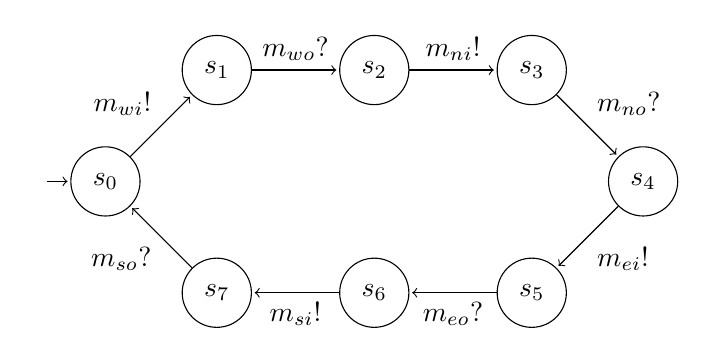
\begin{tikzpicture}[shorten >=1pt,node distance=2cm,on grid,auto,initial distance=0.3cm]
    \node[state, initial left, initial text={}] (S1) {$s_0$};
    \node[state] (S2) [above right of=S1] {$s_1$};
    \node[state] (S3) [right of=S2] {$s_2$};
    \node[state] (S4) [right of=S3] {$s_3$};
    \node[state] (S5) [below right of=S4] {$s_4$};
    \node[state] (S6) [below left of=S5] {$s_5$};
    \node[state] (S7) [left of=S6] {$s_6$};
    \node[state] (S8) [left of=S7] {$s_7$};
    \path[->]
        (S1) edge node {$m_{wi}!$} (S2)
        (S2) edge node {$m_{wo}?$} (S3)
        (S3) edge node {$m_{ni}!$} (S4)
        (S4) edge node {$m_{no}?$} (S5)
        (S5) edge node {$m_{ei}!$} (S6)
        (S6) edge node {$m_{eo}?$} (S7)
        (S7) edge node {$m_{si}!$} (S8)
        (S8) edge node {$m_{so}?$} (S1);
\end{tikzpicture}

% result of composing crossroad with simple environment
\tikzsetnextfilename{cross_simple_res}
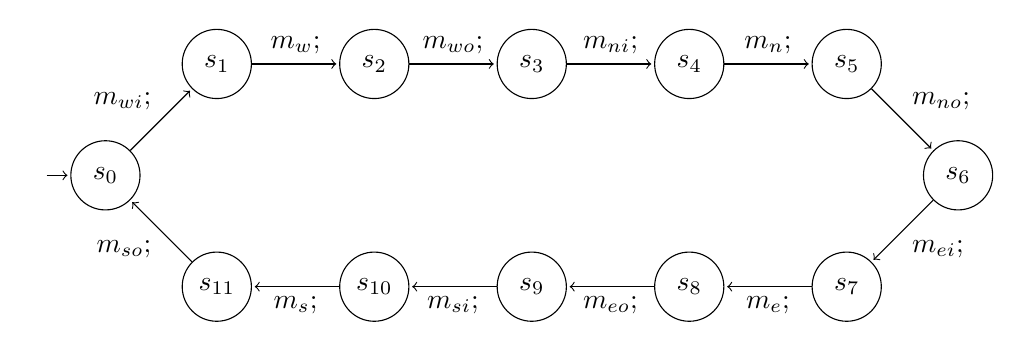
\begin{tikzpicture}[shorten >=1pt,node distance=2cm,on grid,auto,initial distance=0.3cm]
    \node[state, initial left, initial text={}] (S1) {$s_0$};
    \node[state] (S2) [above right of=S1] {$s_1$};
    \node[state] (S3) [right of=S2] {$s_2$};
    \node[state] (S4) [right of=S3] {$s_3$};
    \node[state] (S5) [right of=S4] {$s_4$};
    \node[state] (S6) [right of=S5] {$s_5$};
    \node[state] (S7) [below right of=S6] {$s_6$};
    \node[state] (S8) [below left of=S7] {$s_7$};
    \node[state] (S9) [left of=S8] {$s_8$};
    \node[state] (S10) [left of=S9] {$s_9$};
    \node[state] (S11) [left of=S10] {$s_{10}$};
    \node[state] (S12) [left of=S11] {$s_{11}$};
    \path[->]
        (S1) edge node {$m_{wi};$} (S2)
        (S2) edge node {$m_{w};$} (S3)
        (S3) edge node {$m_{wo};$} (S4)
        (S4) edge node {$m_{ni};$} (S5)
        (S5) edge node {$m_{n};$} (S6)
        (S6) edge node {$m_{no};$} (S7)
        (S7) edge node {$m_{ei};$} (S8)
        (S8) edge node {$m_{e};$} (S9)
        (S9) edge node {$m_{eo};$} (S10)
        (S10) edge node {$m_{si};$} (S11)
        (S11) edge node {$m_{s};$} (S12)
        (S12) edge node {$m_{so};$} (S1);
\end{tikzpicture}

% Process network modelling a crossroad without deadlock
\tikzsetnextfilename{cross_proc_sia}
\begin{tikzpicture}[shorten >=1pt,node distance=2cm,on grid,auto]
    \begin{scope}
        \node[state, initial above, initial text={}] (S1) {$s_0$};
        \node[state] (S2) [above right of=S1] {$s_1$};
        \node[state] (S3) [below left of=S1] {$s_2$};
        \path[->] (S1) [bend left] edge node {$m_{wi}?$} (S2) (S2) [bend left] edge node {$m_{w}!$} (S1);
        \path[->] (S1) [bend right] edge node [swap] {$m_{si}?$} (S3) (S3) [bend right] edge node [swap] {$m_{s}!$} (S1);
        \node[box, fit= (S2) (S3), label={[below, xshift=-19mm]$P'_{\mathit{NW}}$}] (NW) {};
    \end{scope}
    \begin{scope}[xshift=6cm]
        \node[state, initial above, initial text={}] (S1) {$s_3$};
        \node[state] (S2) [above right of=S1] {$s_4$};
        \node[state] (S3) [below left of=S1] {$s_5$};
        \path[->] (S1) [bend left] edge node {$m_{ni}?$} (S2) (S2) [bend left] edge node {$m_{n}!$} (S1);
        \path[->] (S1) [bend right] edge node [swap] {$m_{w}?$} (S3) (S3) [bend right] edge node [swap] {$m_{wo}!$} (S1);
        \node[box, fit= (S2) (S3), label={[below, xshift=-19mm]$P_{\mathit{NE}}$}] (NE) {};
    \end{scope}
    \begin{scope}[yshift=-6cm]
        \node[state, initial above, initial text={}] (S1) {$s_9$};
        \node[state] (S2) [above right of=S1] {$s_{10}$};
        \node[state] (S3) [below left of=S1] {$s_{11}$};
        \path[->] (S1) [bend left] edge node {$m_{s}?$} (S2) (S2) [bend left] edge node {$m_{so}!$} (S1);
        \path[->] (S1) [bend right] edge node [swap] {$m_{e}?$} (S3) (S3) [bend right] edge node [swap] {$m_{eo}!$} (S1);
        \node[box, fit= (S2) (S3), label={[below, xshift=-19mm]$P'_{\mathit{SW}}$}] (SW) {};
    \end{scope}
    \begin{scope}[yshift=-6cm, xshift=6cm]
        \node[state, initial above, initial text={}] (S1) {$s_6$};
        \node[state] (S2) [above right of=S1] {$s_{7}$};
        \node[state] (S3) [below left of=S1] {$s_{8}$};
        \path[->] (S1) [bend left] edge node {$m_{ei}?$} (S2) (S2) [bend left] edge node {$m_{e}!$} (S1);
        \path[->] (S1) [bend right] edge node [swap] {$m_{n}?$} (S3) (S3) [bend right] edge node [swap] {$m_{no}!$} (S1);
        \node[box, fit= (S2) (S3), label={[below, xshift=-19mm]$P_{\mathit{SE}}$}] (SE) {};
    \end{scope}
    \coordinate[right of=NE, xshift=1.5cm] (WO);
    \coordinate[left of=NW, xshift=-1.5cm, yshift=3mm] (WI);
    \coordinate[left of=SW, xshift=-1.5cm] (EO);
    \coordinate[right of=SE, xshift=1.5cm] (EI);
    \coordinate[above of=NW, xshift=27mm, yshift=1.5cm] (SO);
    \coordinate[below of=SW, xshift=-27mm, yshift=-1.5cm] (SI);
    \coordinate[below of=SE, yshift=-1.5cm] (NO);
    \coordinate[above of=NE, yshift=1.5cm] (NI);
    \path[->] (WI) edge node {$m_{wi}$} ([yshift=3mm]NW.west) (NW.east) edge node[xshift=1mm] {$m_{w}$} (NE.west) (NE.east) edge node {$m_{wo}$} (WO);
    \path[->] (EI) edge node [swap]{$m_{ei}$} (SE.east) ([yshift=-3mm]SE.west) edge node[swap] {$m_{e}$} ([yshift=-3mm]SW.east) (SW.west) edge node[swap, xshift=-1mm] {$m_{eo}$} (EO);
    \path[->] (NI) edge node {$m_{ni}$} (NE.north) (NE.south) edge node {$m_{n}$} (SE.north) (SE.south) edge node {$m_{no}$} (NO);
    \path[->] (NW.south) edge node {$m_{s}$} (SW.north);
    \draw[->] (SI) -- node[yshift=-40mm] {$m_{si}$} ([xshift=-3mm, yshift=-3mm]NW.west) |- ([yshift=-3mm]NW.west);
    \draw[->] ([yshift=3mm]SW.east) -| ([xshift=3mm, yshift=3mm]SW.east) -- node[yshift=40mm, swap] {$m_{so}$} (SO);
\end{tikzpicture}

% fifo buffer
\tikzsetnextfilename{sia_fifo}
\begin{tikzpicture}[shorten >=1pt,node distance=2cm,on grid,auto, initial distance=0.3cm]
    \begin{scope}
        \node[state, initial above, initial text={}] (S1) {$s_0$};
        \node[state] (S2) [right of=S1] {$s_1$};
        \node[state] (S3) [right of=S2] {$s_2$};
        \path[->] (S1) [bend left] edge node {$a_{in}?$} (S2);
        \path[->] (S2) [bend left] edge node {$a_{out}!$} (S1);
        \path[->] (S2) [bend left] edge node {$a_{in}?$} (S3);
        \path[->] (S3) [bend left] edge node {$a_{out}!$} (S2);
        \node[box, fit={(S1) (S3) ($(S1.north)+(0,1mm)$) ($(S3.south)-(0,1mm)$)}, label={[below, xshift=23mm]$N_{\mathit{FIFO}}$}] (B) {};
        \coordinate[right of=B, xshift=20mm] (d1);
        \coordinate[left of=B, xshift=-20mm] (d2);
    \end{scope}
    \path[->] (B.east) edge node {$a_{out}$} (d1);
    \path[->] (d2) edge node {$a_{in}$} (B.west);
\end{tikzpicture}

% Process network modelling four connected crossroads
\tikzsetnextfilename{cross_procs_dl}
\begin{tikzpicture}[shorten >=1pt,node distance=2cm,on grid,auto]
    \node[box] (NW) {$C_{\mathit{NW}}$};
    \node[box] (NE) [right of=NW, xshift=1cm] {$C_{\mathit{NE}}$};
    \node[box] (SW) [below of=NW, yshift=-0.5cm] {$C_{\mathit{SW}}$};
    \node[box] (SE) [right of=SW, xshift=1cm] {$C_{\mathit{SE}}$};
    \coordinate[right of=NE, 2up] (nWO);
    \coordinate[left of=NW, 2up] (nWI);
    \coordinate[left of=NW, 2down] (nEO);
    \coordinate[right of=NE, 2down] (nEI);
    \coordinate[right of=SE, 2up] (sWO);
    \coordinate[left of=SW, 2up] (sWI);
    \coordinate[left of=SW, 2down] (sEO);
    \coordinate[right of=SE, 2down] (sEI);
    \coordinate[above of=NW, 2left] (wSO);
    \coordinate[below of=SW, 2left] (wSI);
    \coordinate[above of=NE, 2left] (eSO);
    \coordinate[below of=SE, 2left] (eSI);
    \coordinate[below of=SW, 2right] (wNO);
    \coordinate[above of=NW, 2right] (wNI);
    \coordinate[below of=SE, 2right] (eNO);
    \coordinate[above of=NE, 2right] (eNI);
    \draw[->] (nWI) -- node {$m_{wi_n}$} ([2up]NW.west) ([2up]NE.east) -- node {$m_{wo_n}$} (nWO);
    \draw[->, fifo] ([2up]NW.east) -- node {$m_{w_n}$} ([2up]NE.west);
    \draw[->] (nEI) -- node {$m_{ei_n}$} ([2down]NE.east) ([2down]NW.west) -- node {$m_{eo_n}$} (nEO);
    \draw[->, fifo] ([2down]NE.west) -- node {$m_{e_n}$} ([2down]NW.east);
    \draw[->] (sWI) -- node {$m_{wi_s}$} ([2up]SW.west) ([2up]SE.east) -- node {$m_{wo_s}$} (sWO);
    \draw[->, fifo] ([2up]SW.east) -- node {$m_{w_s}$} ([2up]SE.west);
    \draw[->] (sEI) -- node {$m_{ei_s}$} ([2down]SE.east) ([2down]SW.west) -- node {$m_{eo_s}$} (sEO);
    \draw[->, fifo] ([2down]SE.west) -- node {$m_{e_s}$} ([2down]SW.east);
    \draw[->] (eNI) -- node {$m_{ni_e}$} ([2right]NE.north) ([2right]SE.south) -- node {$m_{no_e}$} (eNO);
    \draw[->, fifo] ([2right]NE.south) -- node {$m_{n_e}$} ([2right]SE.north);
    \draw[->] (wNI) -- node {$m_{ni_w}$} ([2right]NW.north) ([2right]SW.south) -- node {$m_{no_w}$} (wNO);
    \draw[->, fifo] ([2right]NW.south) -- node {$m_{n_w}$} ([2right]SW.north);
    \draw[->] (eSI) -- node {$m_{si_e}$} ([2left]SE.south) ([2left]NE.north) -- node {$m_{so_e}$} (eSO);
    \draw[->, fifo] ([2left]SE.north) -- node {$m_{s_e}$} ([2left]NE.south);
    \draw[->] (wSI) -- node {$m_{si_w}$} ([2left]SW.south) ([2left]NW.north) -- node {$m_{so_w}$} (wSO);
    \draw[->, fifo] ([2left]SW.north) -- node {$m_{s_w}$} ([2left]NW.south);
\end{tikzpicture}

% ================================== tcm.tex ==================================

% single process with SIA where port b1 is decoupled
\tikzsetnextfilename{sia_decoupled}
\begin{tikzpicture}[shorten >=1pt,node distance=2cm,on grid,auto, initial distance=0.3cm]
    \begin{scope}
        \node[state, initial above, initial text={}] (S1) {$s_0$};
        \node[state] (S2) [right of=S1] {$s_1$};
        \node[state] (S3) [above of=S2] {$s_2$};
        \node[state] (S4) [right of=S2] {$s_3$};
        \node[state] (S5) [below of=S2] {$s_4$};
        \path[->] (S1) edge node {$a_1?$} (S2);
        \path[->] (S2) edge node {$\tau_1;$} (S3);
        \path[->] (S2) edge node {$\tau_2;$} (S4);
        \path[->] (S3) edge node [swap] {$b_1!$} (S1);
        \path[->] (S4) edge node {$b_2!$} (S5);
        \path[->] (S5) edge node {$b_3!$} (S1);
        \path[->] (S1) edge [loop left] node {$b_1!$} (S1);
        \path[->] (S2) edge [loop below] node {$b_1!$} (S2);
        \path[->] (S4) edge [loop right] node {$b_1!$} (S4);
        \path[->] (S5) edge [loop below] node {$b_1!$} (S5);
        \node[box, fit= {($(S1.west)-(8mm,0mm)$)($(S4.east)+(8mm,0mm)$)($(S5.south)-(0mm,8mm)$)($(S3.north)+(0mm,0mm)$)}, label={[below, xshift=34mm]$N'_1$}] (B) {};
        \coordinate[right of=B, xshift=30mm, yshift=6mm] (d1);
        \coordinate[right of=B, xshift=30mm] (d2);
        \coordinate[right of=B, xshift=30mm, yshift=-6mm] (d3);
        \coordinate[left of=B, xshift=-30mm, yshift=4mm] (d4);
        \coordinate[left of=B, xshift=-30mm, yshift=-4mm] (d5);
    \end{scope}
    \path[->] ([yshift=6mm] B.east) edge node {$b_1$} (d1);
    \path[->] (B.east) edge node {$b_2$} (d2);
    \path[->] ([yshift=-6mm] B.east) edge node {$b_3$} (d3);
    \path[->] (d4) edge node {$a_1$} ([yshift=4mm] B.west);
    \path[->] (d5) edge node {$a_2$} ([yshift=-4mm] B.west);
\end{tikzpicture}

% decoupler process
\tikzsetnextfilename{sia_decoupler}
\begin{tikzpicture}[shorten >=1pt,node distance=2cm,on grid,auto, initial distance=0.3cm]
    \begin{scope}
        \node[state, initial above, initial text={}] (S1) {$s_5$};
        \path[->] (S1) edge [loop left] node {$a_{in}?$} (S1);
        \path[->] (S1) edge [loop right] node {$a_{out}!$} (S1);
        \node[box, fit= {($(S1.west)-(11mm,4mm)$)($(S1.east)+(11mm,4mm)$)}, label={[below, xshift=17mm]$N_D$}] (B) {};
        \coordinate[right of=B, xshift=10mm] (d1);
        \coordinate[left of=B, xshift=-10mm] (d2);
    \end{scope}
    \path[->] (B.east) edge node {$a_{out}$} (d1);
    \path[->] (d2) edge node {$a_{in}$} (B.west);
\end{tikzpicture}

% result of decoupler composesd with process to decouple port b1
\tikzsetnextfilename{sia_decoupled_res}
\begin{tikzpicture}[shorten >=1pt,node distance=2cm,on grid,auto, initial distance=0.3cm]
    \begin{scope}
        \node[state, initial above, initial text={}] (S1) {$s_{05}$};
        \node[state] (S2) [right of=S1] {$s_{15}$};
        \node[state] (S3) [above of=S2] {$s_{25}$};
        \node[state] (S4) [right of=S2] {$s_{35}$};
        \node[state] (S5) [below of=S2] {$s_{45}$};
        \path[->] (S1) edge node {$a_1?$} (S2);
        \path[->] (S2) edge node {$\tau_1;$} (S3);
        \path[->] (S2) edge node {$\tau_2;$} (S4);
        \path[->] (S3) edge node [swap] {$b_1;$} (S1);
        \path[->] (S4) edge node {$b_2!$} (S5);
        \path[->] (S5) edge node {$b_3!$} (S1);
        \path[->] (S1) edge [loop left] node {$b'_1!$} (S1);
        \path[->] (S2) edge [loop below] node {$b'_1!$} (S2);
        \path[->] (S3) edge [loop above] node {$b'_1!$} (S3);
        \path[->] (S4) edge [loop right] node {$b'_1!$} (S4);
        \path[->] (S5) edge [loop below] node {$b'_1!$} (S5);
        \node[box, fit= {($(S1.west)-(8mm,0mm)$)($(S4.east)+(8mm,0mm)$)($(S5.south)-(0mm,8mm)$)($(S3.north)+(0mm,8mm)$)}, label={[below, xshift=33mm]$\mathit{ND}_1$}] (B) {};
        \coordinate[right of=B, xshift=30mm, yshift=6mm] (d1);
        \coordinate[right of=B, xshift=30mm] (d2);
        \coordinate[right of=B, xshift=30mm, yshift=-6mm] (d3);
        \coordinate[left of=B, xshift=-30mm, yshift=4mm] (d4);
        \coordinate[left of=B, xshift=-30mm, yshift=-4mm] (d5);
    \end{scope}
    \path[->] ([yshift=6mm] B.east) edge node {$b'_1$} (d1);
    \path[->] (B.east) edge node {$b_2$} (d2);
    \path[->] ([yshift=-6mm] B.east) edge node {$b_3$} (d3);
    \path[->] (d4) edge node {$a_1$} ([yshift=4mm] B.west);
    \path[->] (d5) edge node {$a_2$} ([yshift=-4mm] B.west);
\end{tikzpicture}

% fifo with decoupled input
\tikzsetnextfilename{sia_cci_in}
\begin{tikzpicture}[shorten >=1pt,node distance=2cm,on grid,auto, initial distance=0.3cm]
    \begin{scope}
        \node[state, initial above, initial text={}] (S1) {$s_0$};
        \node[state] (S2) [right of=S1] {$s_1$};
        \node[state] (S3) [right of=S2] {$s_2$};
        \path[->] (S1) [bend left] edge node {$a_{in}?$} (S2);
        \path[->] (S2) [bend left] edge node {$a_{out}!$} (S1);
        \path[->] (S2) [bend left] edge node {$a_{in}?$} (S3);
        \path[->] (S3) [bend left] edge node {$a_{out}!$} (S2);
        \path[->] (S3) edge [loop right] node {$a_{in}?$} (S3);
        \node[box, fit={($(S1.west)-(0mm,6mm)$) (S3) ($(S3.east)+(10mm,6mm)$)}, label={[below, xshift=29mm]$N_{\mathit{DIN}}$}] (B) {};
        \coordinate[right of=B, xshift=26mm] (d1);
        \coordinate[left of=B, xshift=-26mm] (d2);
    \end{scope}
    \path[->] (B.east) edge node {$a_{out}$} (d1);
    \path[->] (d2) edge node {$a_{in}$} (B.west);
\end{tikzpicture}

% fifo with decoupled output
\tikzsetnextfilename{sia_cci_out}
\begin{tikzpicture}[shorten >=1pt,node distance=2cm,on grid,auto, initial distance=0.3cm]
    \begin{scope}
        \node[state, initial above, initial text={}] (S1) {$s_0$};
        \node[state] (S2) [right of=S1] {$s_1$};
        \node[state] (S3) [right of=S2] {$s_2$};
        \path[->] (S1) [bend left] edge node {$a_{in}?$} (S2);
        \path[->] (S2) [bend left] edge node {$a_{out}!$} (S1);
        \path[->] (S2) [bend left] edge node {$a_{in}?$} (S3);
        \path[->] (S3) [bend left] edge node {$a_{out}!$} (S2);
        \path[->] (S1) edge [loop left] node {$a_{out}!$} (S1);
        \node[box, fit={(S1) (S3) ($(S1.west)-(11mm,6mm)$) ($(S3.east)+(0,6mm)$)}, label={[below, xshift=28mm]$N_{\mathit{DOUT}}$}] (B) {};
        \coordinate[right of=B, xshift=26mm] (d1);
        \coordinate[left of=B, xshift=-26mm] (d2);
    \end{scope}
    \path[->] (B.east) edge node {$a_{out}$} (d1);
    \path[->] (d2) edge node {$a_{in}$} (B.west);
\end{tikzpicture}

% fifo with decoupled input and output
\tikzsetnextfilename{sia_cci_bi}
\begin{tikzpicture}[shorten >=1pt,node distance=2cm,on grid,auto, initial distance=0.3cm]
    \begin{scope}
        \node[state, initial above, initial text={}] (S1) {$s_0$};
        \node[state] (S2) [right of=S1] {$s_1$};
        \node[state] (S3) [right of=S2] {$s_2$};
        \path[->] (S1) [bend left] edge node {$a_{in}?$} (S2);
        \path[->] (S2) [bend left] edge node {$a_{out}!$} (S1);
        \path[->] (S2) [bend left] edge node {$a_{in}?$} (S3);
        \path[->] (S3) [bend left] edge node {$a_{out}!$} (S2);
        \path[->] (S1) edge [loop left] node {$a_{out}!$} (S1);
        \path[->] (S3) edge [loop right] node {$a_{in}?$} (S3);
        \node[box, fit={(S1) (S3) ($(S1.west)-(11mm,6mm)$) ($(S3.east)+(10mm,6mm)$)}, label={[below, xshift=35mm]$N_{\mathit{DBI}}$}] (B) {};
        \coordinate[right of=B, xshift=32mm] (d1);
        \coordinate[left of=B, xshift=-32mm] (d2);
    \end{scope}
    \path[->] (B.east) edge node {$a_{out}$} (d1);
    \path[->] (d2) edge node {$a_{in}$} (B.west);
\end{tikzpicture}

% temporal firewall
\tikzsetnextfilename{sia_firewall_dec}
\begin{tikzpicture}[shorten >=1pt,node distance=2cm,on grid,auto, initial distance=0.3cm]
    \begin{scope}
        \node[state, initial above, initial text={}] (S1) {$s_0$};
        \node[state] (S2) [above right of=S1] {$s_1$};
        \node[state] (S3) [below right of=S2] {$s_2$};
        \path[->] (S1) edge [swap] node {$p_{clk}?$} (S2);
        \path[->] (S2) edge node {$a_{in}?$} (S3);
        \path[->] (S3) edge node {$a_{out}!$} (S1);
        \node[box, fit={(S1) (S2) (S3)}, label={[below, xshift=19mm]$N_{\mathit{FW}}$}] (B) {};
        \coordinate[right of=B, xshift=17mm] (d1);
        \coordinate[left of=B, xshift=-17mm] (d2);
        \coordinate[left of=B, yshift=-12mm, xshift=-17mm] (d3);
    \end{scope}
    \draw[double,)->] (B.east) -- node {$a_{out}$} (d1);
    \draw[double,->>] (d2) -- node {$a_{in}$} (B.west);
    \path[->] (d3) edge node {$p_{clk}$} ([yshift=-12mm]B.west);
\end{tikzpicture}

% a pnsc with tfs
\tikzsetnextfilename{procs_tf}
\begin{tikzpicture}[shorten >=1pt,node distance=2.5cm,on grid,auto, initial distance=0.3cm]
    \node[box] (S2) {$P_1$};
    \node[box] (S3) [right of=S2] {$P_2$};
    \node[box] (S4) [right of=S3] {$P_3$};
    \coordinate[left of=S2, xshift=5mm, yshift=3mm] (d1);
    \coordinate[left of=S2, xshift=5mm, yshift=-3mm] (d2);
    \coordinate[right of=S4, xshift=-5mm, yshift=3mm] (d3);
    \coordinate[right of=S4, xshift=-5mm, yshift=-3mm] (d4);
    \draw[tf,->] (d1) -- node {\scriptsize $a_1(p_{clk})$ } ([yshift=3mm] S2.west);
    \draw[tf,<-] (d2) -- node {\scriptsize $a_2(p_{clk})$} ([yshift=-3mm] S2.west);
    \draw[tf,->] (d4) -- node [swap] {\scriptsize $a_6(p_{clk})$} ([yshift=-3mm] S4.east);
    \draw[tf,<-] (d3) -- node [swap] {\scriptsize $a_5(p_{clk})$} ([yshift=3mm] S4.east);
    \draw[->] (S3.east) -- node {$a_4$} (S4.west);
    \draw[<-] (S3.west) -- node [swap] {$a_3$} (S2.east);
\end{tikzpicture}

% a complete tt pnsc with tfs
\tikzsetnextfilename{procs_tt}
\begin{tikzpicture}[shorten >=1pt,node distance=2.7cm,on grid,auto, initial distance=0.3cm]
    \node[box] (S2) {$P_1$};
    \node[box] (S3) [right of=S2] {$P_2$};
    \node[box] (S4) [right of=S3] {$P_3$};
    \coordinate[left of=S2, xshift=7mm, yshift=3mm] (d1);
    \coordinate[left of=S2, xshift=7mm, yshift=-3mm] (d2);
    \coordinate[right of=S4, xshift=-7mm, yshift=3mm] (d3);
    \coordinate[right of=S4, xshift=-7mm, yshift=-3mm] (d4);
    \draw[tf,->] (d1) -- node {\scriptsize $a_1(p_{clk})$ } ([yshift=3mm] S2.west);
    \draw[tf,<-] (d2) -- node {\scriptsize $a_2(p_{clk})$} ([yshift=-3mm] S2.west);
    \draw[tf,->] (d4) -- node [swap] {\scriptsize $a_6(p_{clk})$} ([yshift=-3mm] S4.east);
    \draw[tf,<-] (d3) -- node [swap] {\scriptsize $a_5(p_{clk})$} ([yshift=3mm] S4.east);
    \draw[tf,->] (S3.east) -- node {\scriptsize $a_4(p_{clk})$} (S4.west);
    \draw[tf,<-] (S3.west) -- node [swap] {\scriptsize $a_3(p_{clk})$} (S2.east);
\end{tikzpicture}

% a tt pnsc with asynchronous tfs
\tikzsetnextfilename{procs_tt_async}
\begin{tikzpicture}[shorten >=1pt,node distance=2cm,on grid,auto, initial distance=0.3cm]
    \node[box] (S2) {$P_1$};
    \coordinate[left of=S2] (d1);
    \coordinate[right of=S2] (d2);
    \node[box] (S3) [right of=d2] {$P_2$};
    \coordinate[right of=S3] (d3);
    \draw[tf,->] (d1) -- node {\scriptsize $a_1(clk_1)$ } (S2.west);
    \draw[tf,->] (S2.east) -- node {\scriptsize $a_2(clk_1)$ } (d2);
    \draw[tf,->] (d2) -- node {\scriptsize $a_2(clk_2)$ } (S3.west);
    \draw[tf,->] (S3.east) -- node {\scriptsize $a_3(clk_2)$ } (d3);
\end{tikzpicture}

% mixed-criticality pnsc
\tikzstyle{sstate}=[state, minimum size=0pt, fill=black]
\tikzsetnextfilename{mc_pnsc_ex}
\begin{tikzpicture}[shorten >=1pt,node distance=1.5cm,on grid,auto, initial distance=0.3cm]
    \begin{scope}
        \node[sstate, initial above, initial text={}] (S1) {};
        \path[->] (S1) edge [loop right] node {$cam!$} (S1);
        \node[box, fit= {(S1)($(S1.east)+(13mm,3mm)$)($(S1.west)-(0,3mm)$)}, label={[below, xshift=9mm]$P_{cam}$}] (CAM) {};
    \end{scope}
    \begin{scope}[xshift=45mm]
        \node[sstate, initial above, initial text={}] (S1) {};
        \node[sstate] (S2) [above right of=S1] {};
        \node[sstate] (S3) [below right of=S1] {};
        \path[->] (S1) edge node {$cam?$} (S2);
        \path[->] (S2) edge node {$f_1!$} (S3);
        \path[->] (S3) edge node {$f_2!$} (S1);
        \node[box, fit= {(S1)(S2)(S3)}, label={[below, xshift=-7mm]$P_{copy}$}] (CPY) {};
    \end{scope}
    \begin{scope}[xshift=84mm, yshift=15mm]
        \node[sstate, initial above, initial text={}] (S1) {};
        \node[sstate] (S2) [right of=S1] {};
        \path[->] (S1) [bend left] edge node {$f_1?$} (S2);
        \path[->] (S2) [bend left] edge node {$vf!$} (S1);
        \node[box, line width=1pt, inner sep=2mm, fit= {($(S1)-(5mm,7mm)$)($(S2)+(5mm,7mm)$)}, label={[below, xshift=9mm]$P_{filter}$}] (VF) {};
    \end{scope}
    \begin{scope}[xshift=84mm, yshift=-15mm]
        \node[sstate, initial above, initial text={}] (S1) {};
        \node[sstate] (S2) [right of=S1] {};
        \path[->] (S1) [bend left] edge node {$f_2?$} (S2);
        \path[->] (S2) [bend left] edge node {$fd!$} (S1);
        \node[box, inner sep=2mm, fit= {($(S1)-(5mm,7mm)$)($(S2)+(5mm,7mm)$)}, label={[below, xshift=11mm]$P_{fd}$}] (FD) {};
    \end{scope}
    \begin{scope}[xshift=126mm]
        \node[sstate, initial above, initial text={}] (S1) {};
        \node[sstate] (S2) [above right of=S1] {};
        \node[sstate] (S3) [below right of=S1] {};
        \path[->] (S1) edge node {$vf?$} (S2);
        \path[->] (S2) edge node {$fd?$} (S3);
        \path[->] (S3) edge node {$res!$} (S1);
        \node[box, fit= {(S1)(S2)(S3)($(S3.east)+(1mm,0)$)}, label={[below, xshift=-6mm]$P_{merge}$}] (MRG) {};
    \end{scope}
    \begin{scope}[xshift=163mm]
        \node[sstate, initial above, initial text={}] (S1) {};
        \path[->] (S1) edge [loop right] node {$res?$} (S1);
        \node[box, fit= {(S1)($(S1.east)+(12mm,3mm)$)($(S1.west)-(0mm,3mm)$)}, label={[below, xshift=7mm]$P_{screen}$}] (SCRN) {};
    \end{scope}
    \draw[dashed,double,->] (CAM.east) -- node {$cam(\frac{1}{24})$} (CPY.west);
    \draw[double,->] ([yshift=15mm]CPY.east) -- node {$f_1$} (VF.west);
    \draw[double,->] (VF.east) -- node {$vf$} ([yshift=15mm]MRG.west);
    \draw[dashed,double,)->] ([yshift=-15mm]CPY.east) -- node {$f_2(\frac{1}{5})$} (FD.west);
    \draw[double,->>] (FD.east) -- node {$fd$} ([yshift=-15mm]MRG.west);
    \draw[double,->] (MRG.east) -- node {$res$} (SCRN.west);
\end{tikzpicture}

%==================================== block.tex ===============================

% Example of a lonely blocker
\tikzsetnextfilename{sia_lb}
\begin{tikzpicture}[shorten >=1pt,node distance=2cm,on grid,auto, initial distance=0.3cm]
    \begin{scope}
        \node[state, initial above, initial text={}] (S1) {$s_0$};
        \node[state] (S2) [above right of=S1] {$s_1$};
        \node[state] (S3) [below right of=S1] {$s_2$};
        \path[->] (S1) edge node {$a!$} (S2);
        \path[->] (S1) edge node [swap] {$c?$} (S3);
        \node[box, fit= (S1) (S2) (S3), label={[below, xshift=-13mm]$M_2$}] (B1) {};
    \end{scope}
    \begin{scope}[xshift=4.8cm]
        \node[state, initial above, initial text={}] (S1) {$s_3$};
        \node[state] (S2) [above right of=S1] {$s_4$};
        \node[state] (S3) [below right of=S1] {$s_5$};
        \path[->] (S1) edge node {$a?$} (S2);
        \path[->] (S1) edge node [swap] {$b!$} (S3);
        \node[box, fit= (S1) (S2) (S3), label={[below, xshift=-13mm]$N_2$}] (B2) {};
    \end{scope}
    \coordinate[left of=B1, xshift=-10mm] (d);
    \path[->] ([yshift=5mm]B1.east) edge node {$a$} ([yshift=5mm]B2.west);
    \path[->] ([yshift=-5mm]B2.west) edge node [swap] {$b$} ([yshift=-5mm]B1.east);
    \path[->] (d) edge node {$c$} (B1.west);
\end{tikzpicture}

% example of processes where sias have cycles
\tikzsetnextfilename{sia_pnsc_cycles}
\begin{tikzpicture}[shorten >=1pt,node distance=2cm,on grid,auto,initial distance=0.3cm]
    \begin{scope}
        \node[state, initial above, initial text={}] (S1) {$s_0$};
        \node[state] (S2) [right of=S1] {$s_1$};
        \path[->]
            (S1) edge [bend left] node {$a!$} (S2)
            (S2) edge [bend left] node {$b?$} (S1);
        \node[box, fit= (S1) (S2), label={[below, xshift=16mm]$O_1$}] (B1) {};
    \end{scope}
    \begin{scope}[xshift=4.8cm]
        \node[state, initial above, initial text={}] (S1) {$s_2$};
        \path[->] (S1) edge [loop right] node {$\tau_1;$} (S1);
        \coordinate[right of=S1, xshift=-0.8cm] (dt);
        \node[box, fit= (S1) (dt), label={[below, xshift=10mm]$O_2$}] (B2) {};
    \end{scope}
    \begin{scope}[yshift=-2.3cm]
        \node[state, initial above, initial text={}] (S1) {$s_3$};
        \node[state] (S2) [right of=S1] {$s_4$};
        \path[->]
            (S1) edge [bend left] node {$c!$} (S2)
            (S2) edge [bend left] node {$d!$} (S1);
        \node[box, fit= (S1) (S2), label={[below, xshift=16mm]$O_3$}] (B3) {};
    \end{scope}
    \begin{scope}[yshift=-2.3cm, xshift=4.8cm]
        \node[state, initial above, initial text={}] (S1) {$s_5$};
        \node[state] (S2) [right of=S1] {$s_6$};
        \path[->]
            (S1) edge [bend left] node {$d?$} (S2)
            (S2) edge [bend left] node {$c?$} (S1);
        \node[box, fit= (S1) (S2), label={[below, xshift=16mm]$O_4$}] (B4) {};
    \end{scope}
    \path[->]
        ([yshift=2mm] B1.east) edge node {$a$} ([yshift=2mm] B2.west)
        ([yshift=-2mm] B2.west) edge node {$b$} ([yshift=-2mm] B1.east);
    \path[->]
        ([yshift=2mm] B3.east) edge node {$c$} ([yshift=2mm] B4.west)
        ([yshift=-2mm] B3.east) edge node [swap] {$d$} ([yshift=-2mm] B4.west);
\end{tikzpicture}

%=================================== streamix.tex =============================

% diverging node
\tikzsetnextfilename{sia_fc_div}
\begin{tikzpicture}[shorten >=1pt,node distance=2cm,on grid,auto, initial distance=0.3cm]
    \begin{scope}
        \node[state, initial above, initial text={}] (S1) {$s_0$};
        \node[state] (S2) [above right of=S1] {$s_2$};
        \node[state] (S3) [below right of=S2] {$s_1$};
        \path[->] (S1) edge node {$a?$} (S3);
        \path[->] (S3) edge [swap] node {$b!$} (S2);
        \path[->] (S2) edge [swap] node {$c!$} (S1);
        \node[box, fit= (S1) (S2) (S3), label={[below, xshift=19mm]$N_{div}$}] (B) {};
        \coordinate[right of=B, xshift=14mm, yshift=6mm] (d1);
        \coordinate[right of=B, xshift=14mm, yshift=-6mm] (d2);
        \coordinate[left of=B, xshift=-14mm] (d3);
    \end{scope}
    \path[->] ([yshift=6mm]B.east) edge node {$b$} (d1);
    \path[->] ([yshift=-6mm]B.east) edge node {$c$} (d2);
    \path[->] (d3) edge node {$a$} (B.west);
\end{tikzpicture}

% summing node
\tikzsetnextfilename{sia_fc_sum}
\begin{tikzpicture}[shorten >=1pt,node distance=2cm,on grid,auto, initial distance=0.3cm]
    \begin{scope}
        \node[state, initial above, initial text={}] (S1) {$s_0$};
        \node[state] (S2) [right of=S1] {$s_1$};
        \node[state] (S3) [left of=S1] {$s_2$};
        \path[->] (S1) [bend left] edge node {$a?$} (S2);
        \path[->] (S2) [bend left] edge node {$c!$} (S1);
        \path[->] (S1) [bend right] edge [swap] node {$b?$} (S3);
        \path[->] (S3) [bend right] edge [swap] node {$c!$} (S1);
        \node[box, fit={(S1) (S2) (S3)($(S1.north)+(-17mm,3mm)$) ($(S3.south)+(0,-3mm)$)}, label={[below, xshift=24mm]$N_{sum}$}] (B) {};
        \coordinate[right of=B, xshift=19mm] (d1);
        \coordinate[left of=B, xshift=-19mm, yshift=6mm] (d2);
        \coordinate[left of=B, xshift=-19mm, yshift=-6mm] (d3);
    \end{scope}
    \path[->] (B.east) edge node {$c$} (d1);
    \path[->] (d2) edge node {$a$} ([yshift=6mm]B.west);
    \path[->] (d3) edge node {$b$} ([yshift=-6mm]B.west);
\end{tikzpicture}

% combined summing and diverging node
\tikzsetnextfilename{sia_fc_full}
\begin{tikzpicture}[shorten >=1pt,node distance=2cm,on grid,auto, initial distance=0.3cm]
    \begin{scope}
        \node[state, initial above, initial text={}] (S1) {$s_0$};
        \node[state] (S2) [above right of=S1] {$s_2$};
        \node[state] (S3) [below right of=S2] {$s_1$};
        \node[state] (S4) [above left of=S1] {$s_4$};
        \node[state] (S5) [below left of=S4] {$s_3$};
        \path[->] (S1) edge node {$a?$} (S3);
        \path[->] (S3) edge [swap] node {$c!$} (S2);
        \path[->] (S2) edge [swap] node {$d!$} (S1);
        \path[->] (S1) edge [swap] node {$b?$} (S5);
        \path[->] (S5) edge node {$c!$} (S4);
        \path[->] (S4) edge node {$d!$} (S1);
        \node[box, fit={(S3) (S2) (S5)}, label={[below, xshift=32mm]$N_{full}$}] (B) {};
        \coordinate[left of=B, xshift=-29mm, yshift=6mm] (d1);
        \coordinate[left of=B, xshift=-29mm, yshift=-6mm] (d2);
        \coordinate[right of=B, xshift=29mm, yshift=6mm] (d3);
        \coordinate[right of=B, xshift=29mm, yshift=-6mm] (d4);
    \end{scope}
    \path[->] (d1) edge node {$a$} ([yshift=6mm]B.west);
    \path[->] (d2) edge node {$b$} ([yshift=-6mm]B.west);
    \path[->] ([yshift=6mm]B.east) edge node {$c$} (d3);
    \path[->] ([yshift=-6mm]B.east) edge node {$d$} (d4);
\end{tikzpicture}

% a tt pnsc with asynchronous tfs
\tikzsetnextfilename{net_tt1}
\begin{tikzpicture}[shorten >=1pt,node distance=2cm,on grid,auto, initial distance=0.3cm]
    \node[box] (S2) {$N_1$};
    \coordinate[left of=S2] (d1);
    \node[box] (S3) [right of=S2, xshift=7mm] {$N_2$};
    \coordinate[right of=S3] (d3);
    \draw[tf,->] (d1) -- node {\scriptsize $x(clk)$ } (S2.west);
    \draw[tf,->] (S2.east) -- node {\scriptsize $y(clk)$ } (S3.west);
    \draw[tf,->] (S3.east) -- node {\scriptsize $z(clk)$ } (d3);
\end{tikzpicture}

% a tt pnsc with asynchronous tfs
\tikzsetnextfilename{net_tt2}
\begin{tikzpicture}[shorten >=1pt,node distance=2cm,on grid,auto, initial distance=0.3cm]
    \node[box] (S2) {$N_1$};
    \coordinate[left of=S2] (d1);
    \coordinate[right of=S2] (d2);
    \node[box] (S3) [right of=d2] {$N_2$};
    \coordinate[right of=S3] (d3);
    \draw[tf,->] (d1) -- node {\scriptsize $x(clk_1)$ } (S2.west);
    \draw[tf,->] (S2.east) -- node {\scriptsize $y(clk_1)$ } (d2);
    \draw[tf,->] (d2) -- node {\scriptsize $y(clk_2)$ } (S3.west);
    \draw[tf,->] (S3.east) -- node {\scriptsize $z(clk_2)$ } (d3);
\end{tikzpicture}

%========================= rts.tex ============================================

% toolchain of streamix
\newcommand*{\XDelta}{3.5}%
\newcommand*{\YDelta}{2.5}%
\pgfdeclarelayer{bg}    % declare background layer
\pgfsetlayers{bg,main}  % set the order of the layers (main is the standard layer)
\tikzsetnextfilename{toolchain}
\begin{tikzpicture}[align=center]
    \path   (0, 0)                  node        (inSmx)     {Streamix \\ input program}
            +(\XDelta, 0)           node        (inSia)     {SIAs of \\ boxes*}
            +(-\XDelta, 0)          node        (inBox)     {Box \\ implementations}
            ++(0, -\YDelta)         node[boxr]  (smxc)      {1. Streamix \\ compiler \\ \texttt{smxc} }
            ++(0, -\YDelta)         node[boxr]  (rtsp)      {2. Streamix RTS \\ preprocessor \\ \texttt{smxrtsp} }
            +(-2*\XDelta, 0)        node (rts)              {Streamix \\ RTS library}
            +(-\XDelta, -\YDelta)   node[boxr]  (gcc)       {4. C compiler}
            +(\XDelta, -\YDelta)    node[boxr]  (sia)       {3. SIA checker \\ \texttt{smxsia} }
            +(-\XDelta, -2*\YDelta) node        (outBox)    {Executable \\ program}
            +(\XDelta, -2*\YDelta)  node        (outSia)    {Yes / No};
    \begin{pgfonlayer}{bg}    % select the background layer
        \node[boxbg, fit= (inSmx) (inSia) (inBox)] (B) {};
    \end{pgfonlayer}
    \path[->] (inSmx.south) edge (smxc.north);
    \draw[->] (inSia.south) -- ([yshift=-5mm]inSia.south) -| ([xshift=3mm]smxc.north);
    \path[->] (smxc.south) edge (rtsp.north);
    \draw[->] (smxc.east) -| (sia.north);
    \draw[->] (rtsp.east) -| ([xshift=-3mm]sia.north);
    \draw[->] (rtsp.south) |- ([xshift=3mm,yshift=5mm]gcc.north) -- ([xshift=3mm]gcc.north);
    \draw[->] (rts.south) |- ([xshift=-3mm,yshift=5mm]gcc.north) -| ([xshift=-3mm]gcc.north);
    \draw[->] (inBox.south) -- (gcc.north);
    \path[->] (gcc.south) edge (outBox.north);
    \path[->] (sia.south) edge (outSia.north);
\end{tikzpicture}

%=============================== UNUSED =======================================

\tikzsetnextfilename{ccis}
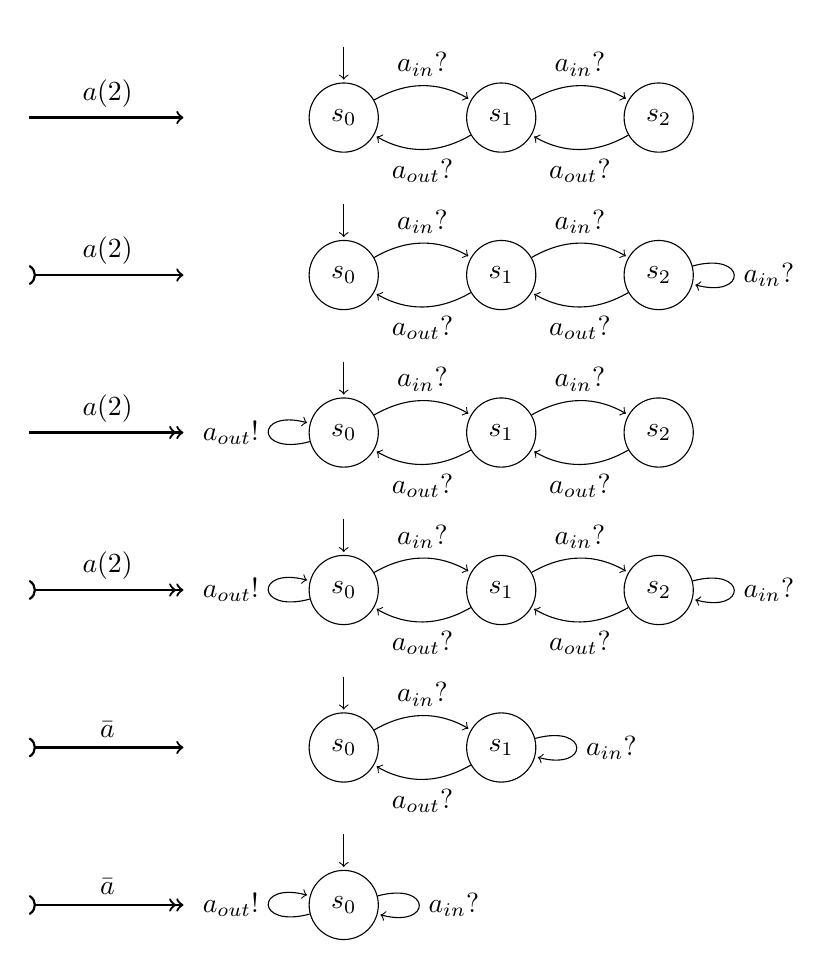
\begin{tikzpicture}[shorten >=1pt,node distance=2cm,on grid,auto]
    \coordinate (L1);
    \coordinate[right of=L1] (R1);
    \draw[thick, ->] (L1) -- node {$a(2)$} (R1);
    \begin{scope}
        \node[state, initial above, initial text={}] (S1) [right of=R1] {$s_0$};
        \node[state] (S2) [right of=S1] {$s_1$};
        \node[state] (S3) [right of=S2] {$s_2$};
        \path[->] (S1) [bend left] edge node {$a_{in}?$} (S2);
        \path[->] (S2) [bend left] edge node {$a_{out}?$} (S1);
        \path[->] (S2) [bend left] edge node {$a_{in}?$} (S3);
        \path[->] (S3) [bend left] edge node {$a_{out}?$} (S2);
    \end{scope}
    \coordinate[below of=L1] (L2);
    \coordinate[right of=L2] (R2);
    \draw[thick, )->] (L2) -- node {$a(2)$} (R2);
    \begin{scope}
        \node[state, initial above, initial text={}] (S1) [right of=R2] {$s_0$};
        \node[state] (S2) [right of=S1] {$s_1$};
        \node[state] (S3) [right of=S2] {$s_2$};
        \path[->] (S1) [bend left] edge node {$a_{in}?$} (S2);
        \path[->] (S2) [bend left] edge node {$a_{out}?$} (S1);
        \path[->] (S2) [bend left] edge node {$a_{in}?$} (S3);
        \path[->] (S3) [bend left] edge node {$a_{out}?$} (S2);
        \path[->] (S3) edge [loop right] node {$a_{in}?$} (S3);
    \end{scope}
    \coordinate[below of=L2] (L3);
    \coordinate[right of=L3] (R3);
    \draw[thick, ->>] (L3) -- node {$a(2)$} (R3);
    \begin{scope}
        \node[state, initial above, initial text={}] (S1) [right of=R3] {$s_0$};
        \node[state] (S2) [right of=S1] {$s_1$};
        \node[state] (S3) [right of=S2] {$s_2$};
        \path[->] (S1) [bend left] edge node {$a_{in}?$} (S2);
        \path[->] (S2) [bend left] edge node {$a_{out}?$} (S1);
        \path[->] (S2) [bend left] edge node {$a_{in}?$} (S3);
        \path[->] (S3) [bend left] edge node {$a_{out}?$} (S2);
        \path[->] (S1) edge [loop left] node {$a_{out}!$} (S1);
    \end{scope}
    \coordinate[below of=L3] (L4);
    \coordinate[right of=L4] (R4);
    \draw[thick, )->>] (L4) -- node {$a(2)$} (R4);
    \begin{scope}
        \node[state, initial above, initial text={}] (S1) [right of=R4] {$s_0$};
        \node[state] (S2) [right of=S1] {$s_1$};
        \node[state] (S3) [right of=S2] {$s_2$};
        \path[->] (S1) [bend left] edge node {$a_{in}?$} (S2);
        \path[->] (S2) [bend left] edge node {$a_{out}?$} (S1);
        \path[->] (S2) [bend left] edge node {$a_{in}?$} (S3);
        \path[->] (S3) [bend left] edge node {$a_{out}?$} (S2);
        \path[->] (S1) edge [loop left] node {$a_{out}!$} (S1);
        \path[->] (S3) edge [loop right] node {$a_{in}?$} (S3);
    \end{scope}
    \coordinate[below of=L4] (L5);
    \coordinate[right of=L5] (R5);
    \draw[thick, )->] (L5) -- node {$\bar a$} (R5);
    \begin{scope}
        \node[state, initial above, initial text={}] (S1) [right of=R5] {$s_0$};
        \node[state] (S2) [right of=S1] {$s_1$};
        \path[->] (S1) [bend left] edge node {$a_{in}?$} (S2);
        \path[->] (S2) [bend left] edge node {$a_{out}?$} (S1);
        \path[->] (S2) edge [loop right] node {$a_{in}?$} (S2);
    \end{scope}
    \coordinate[below of=L5] (L6);
    \coordinate[right of=L6] (R6);
    \draw[thick, )->>] (L6) -- node {$\bar a$} (R6);
    \begin{scope}
        \node[state, initial above, initial text={}] (S1) [right of=R6] {$s_0$};
        \path[->] (S1) edge [loop left] node {$a_{out}!$} (S1);
        \path[->] (S1) edge [loop right] node {$a_{in}?$} (S1);
    \end{scope}
\end{tikzpicture}

% time-triggered wrapper sia
\tikzsetnextfilename{sia_tt}
\begin{tikzpicture}[shorten >=1pt,node distance=2cm,on grid,auto, initial distance=0.3cm]
    \begin{scope}
        \node[state, initial above, initial text={}] (S1) {$s_0$};
        \node[state] (S2) [above right of=S1] {$s_1$};
        \node[state] (S3) [below right of=S2] {$s_2$};
        \path[->] (S1) edge [swap] node {$clk?$} (S2);
        \path[->] (S2) edge node {$a!$} (S3);
        \path[->] (S3) edge node {$b?$} (S1);
        \path[->] (S1) edge [loop left] node {$b_{tt}!$} (S1);
        \path[->] (S1) edge [loop below] node {$a_{tt}?$} (S1);
        \path[->] (S2) edge [loop left] node {$b_{tt}!$} (S2);
        \path[->] (S2) edge [loop above] node {$a_{tt}?$} (S2);
        \path[->] (S3) edge [loop right] node {$b_{tt}!$} (S3);
        \path[->] (S3) edge [loop below] node {$a_{tt}?$} (S3);
        \node[box, inner sep=13mm, fit= (S1) (S2) (S3), label={[below, xshift=27mm]$N_{tt}$}] (B) {};
        \coordinate[right of=B, xshift=24mm] (d1);
        \coordinate[left of=B, xshift=-24mm] (d2);
        \coordinate[left of=B, yshift=-18mm, xshift=-24mm] (d3);
    \end{scope}
    \path[)->] (B.east) edge node {$b_{tt}$} (d1);
    \path[->>] (d2) edge node {$a_{tt}$} (B.west);
    \path[->] (d3) edge node {$clk$} ([yshift=-18mm]B.west);
\end{tikzpicture}

% event bounded buffer
\tikzsetnextfilename{sia_etb_mirt}
\begin{tikzpicture}[shorten >=1pt,node distance=2.8cm,on grid,auto, initial distance=0.3cm]
    \begin{scope}
        \node[state, initial above, initial text={}] (S1) {$s_0$};
        \node[state] (S2) [right of=S1] {$s_1$};
        \node[state] (S3) [right of=S2] {$s_2$};
        \coordinate[right of=S3, xshift=3mm] (d01);
        \coordinate[above right of=S1] (d02);
        \coordinate[below right of=S1] (d03);
        \coordinate[left of=S1, xshift=-3mm] (d04);
        \path[->] (S1) edge[loop left] node[align=center] {$a_{in}?$\\$\{0 \leq x < \infty\}^\epsilon$\\$\{\}$} (S1);
        \path[->] (S1) edge[bend left] node[align=center] {$a_{out}!$\\$\{0 \leq x < \infty\}^\epsilon$\\$\{x\}$} (S2);
        \path[->] (S2) edge[bend left] node[align=center] {$a_{in}?$\\$\{0 \leq x < t_{nr}\}^\epsilon$\\$\{\}$} (S3);
        \path[->] (S3) edge[loop right] node[align=center] {$a_{in}?$\\$\{0 \leq x < t_{nr}\}^\epsilon$\\$\{\}$} (S3);
        \path[->] (S3) edge[bend left] node[align=center] {$a_{out}!$\\$\{t_{nr} \leq x < \infty\}^\epsilon$\\$\{x\}$} (S2);
        \path[->] (S2) edge[bend left] node[align=center] {$a_{in}?$\\$\{t_{nr} \leq x < \infty\}^\epsilon$\\$\{\}$} (S1);
        \node[box, fit= (d04) (d02) (d03) (d01), label={[below, xshift=56mm]$N_{\mathit{MIRT}}$}] (B) {};
        \coordinate[right of=B, xshift=46mm] (d1);
        \coordinate[left of=B, xshift=-46mm] (d2);
    \end{scope}
    \path[->] (B.east) edge node {$a_{out}$} (d1);
    \path[->>] (d2) edge node {$a_{in}$} (B.west);
\end{tikzpicture}

% temporal firewall
\tikzsetnextfilename{sia_firewall}
\begin{tikzpicture}[shorten >=1pt,node distance=2cm,on grid,auto, initial distance=0.3cm]
    \begin{scope}
        \node[state, initial above, initial text={}] (S1) {$s_0$};
        \path[->] (S1) edge [loop left] node {$a_{in}?$} (S1);
        \path[->] (S1) edge [loop right] node {$a'_{in}!$} (S1);
        \node[box, fit= {($(S1.west)-(13mm,6mm)$)($(S1.east)+(13mm,6mm)$)}, label={[below, xshift=17mm]$N_D$}] (B1) {};
        \coordinate[left of=B1, xshift=-10mm] (d1);
    \end{scope}
    \begin{scope}[xshift=40mm]
        \node[state, initial left, initial text={}] (S1) {$s_0$};
        \node[state] (S2) [above right of=S1] {$s_1$};
        \node[state] (S3) [below right of=S1] {$s_2$};
        \path[->] (S1) edge node {$p_{clk}?$} (S2);
        \path[->] (S2) edge node {$a'_{in}?$} (S3);
        \path[->] (S3) edge node {$a'_{out}!$} (S1);
        \node[box, inner sep=5mm, fit={(S1) (S2) (S3)}, label={[below, xshift=-11mm]$N_{\mathit{FW}}$}] (B) {};
        \coordinate[left of=B, yshift=-20mm, xshift=-07mm] (d3);
    \end{scope}
    \begin{scope}[xshift=94mm]
        \node[state, initial above, initial text={}] (S1) {$s_0$};
        \path[->] (S1) edge [loop left] node {$a'_{out}?$} (S1);
        \path[->] (S1) edge [loop right] node {$a_{out}!$} (S1);
        \node[box, fit= {($(S1.west)-(13mm,6mm)$)($(S1.east)+(13mm,6mm)$)}, label={[below, xshift=17mm]$N_D$}] (B2) {};
        \coordinate[right of=B2, xshift=10mm] (d2);
    \end{scope}
    \path[->] (d1) edge node {$a_{in}$} (B1.west);
    \path[->] (B1.east) edge node {$a'_{in}$} (B.west);
    \path[->] (B.east) edge node {$a'_{out}$} (B2.west);
    \path[->] (B2.east) edge node {$a_{out}$} (d2);
    \path[->] (d3) edge node {$p_{clk}$} ([yshift=-20mm]B.west);
\end{tikzpicture}

% a pnsc with tfs
\tikzsetnextfilename{procs_tf_tmp}
\begin{tikzpicture}[shorten >=1pt,node distance=2cm,on grid,auto, initial distance=0.3cm]
    \node[box] (S2) {$P_1$};
    \node[box] (S11) [left of=S2, xshift=-3mm, yshift=6mm]{$\mathit{TF}(a_1)$};
    \node[box] (S12) [left of=S2, xshift=-3mm, yshift=-6mm]{$\mathit{TF}(a_2)$};
    \node[box] (S3) [right of=S2] {$P_2$};
    \node[box] (S4) [right of=S3] {$P_3$};
    \node[box] (S51) [right of=S4, xshift=3mm, yshift=6mm] {$\mathit{TF}(a_5)$};
    \node[box] (S52) [right of=S4, xshift=3mm, yshift=-6mm] {$\mathit{TF}(a_6)$};
    \coordinate[left of=S11, xshift=3mm] (d1);
    \coordinate[left of=S12, xshift=3mm] (d2);
    \coordinate[right of=S51, xshift=-3mm] (d3);
    \coordinate[right of=S52, xshift=-3mm] (d4);
    \coordinate[left of=S12, xshift=3mm, yshift=-10mm] (d5);
    \path[->] (d1) edge node {$a_1$} (S11.west);
    \path[->] (S11.east) edge node {$a'_1$} ([yshift=2mm] S2.west);
    \path[<-] (d2) edge node {$a_2$} (S12.west);
    \path[<-] (S12.east) edge node [swap] {$a'_2$} ([yshift=-2mm] S2.west);
    \path[->] (d3) edge node [swap] {$a_6$} (S51.east);
    \path[->] ([yshift=2mm] S4.east) edge node {$a'_5$} (S51.west);
    \path[<-] (d4) edge node [swap] {$a_5$} (S52.east);
    \path[<-] ([yshift=-2mm] S4.east) edge node [swap] {$a'_6$} (S52.west);
    \path[->] (S3.east) edge node {$a_4$} (S4.west);
    \path[->] (S3.west) edge node [swap] {$a_3$} (S2.east);
    \draw[->] (d5) -| node[yshift=3mm] {$clk$} ([xshift=-2mm, yshift=-3mm] S11.west) -- ([yshift=-3mm] S11.west);
    \draw[->] ([xshift=-2mm, yshift=-3mm] S12.west) -- ([yshift=-3mm] S12.west);
    \draw[->] (d5) -| ([xshift=-2mm, yshift=-3mm] S51.west) -- ([yshift=-3mm] S51.west);
    \draw[->] ([xshift=-2mm, yshift=-3mm] S52.west) -- ([yshift=-3mm] S52.west);
\end{tikzpicture}

\end{document}
